% \iffalse
\let\negmedspace\undefined
\let\negthickspace\undefined
\documentclass[journal,12pt,twocolumn]{IEEEtran}
\usepackage{cite}
\usepackage{amsmath,amssymb,amsfonts,amsthm}
\usepackage{algorithmic}
\usepackage{graphicx}
\usepackage{textcomp}
\usepackage{xcolor}
\usepackage{txfonts}
\usepackage{listings}
\usepackage{enumitem}
\usepackage{mathtools}
\usepackage{gensymb}
\usepackage{comment}
\usepackage[breaklinks=true]{hyperref}
\usepackage{tkz-euclide}
\usepackage{listings}
\usepackage{gvv}
\def\inputGnumericTable{}
\usepackage[latin1]{inputenc}
\usepackage{color}
\usepackage{array}
\usepackage{longtable}
\usepackage{calc}
\usepackage{multirow}
\usepackage{hhline}
\usepackage{ifthen}
\usepackage{lscape}

\newtheorem{theorem}{Theorem}[section]
\newtheorem{problem}{Problem}
\newtheorem{proposition}{Proposition}[section]
\newtheorem{lemma}{Lemma}[section]
\newtheorem{corollary}[theorem]{Corollary}
\newtheorem{example}{Example}[section]
\newtheorem{definition}[problem]{Definition}
\newcommand{\BEQA}{\begin{eqnarray}}
\newcommand{\EEQA}{\end{eqnarray}}
\newcommand{\define}{\stackrel{\triangle}{=}}
\theoremstyle{remark}
\newtheorem{rem}{Remark}
\begin{document}

\bibliographystyle{IEEEtran}
\vspace{3cm}

\title{GATE 2022  -AE 63}
\author{EE23BTECH11057 - Shakunaveti Sai Sri Ram Varun$^{}$% &lt;-this % stops a space
}
\maketitle
\newpage
\bigskip
\vspace{2cm}
\textbf{Question: }
Which one of the following is the closed form for the generating function of the sequence $ \bigl\{ a \bigl\}_{n \geq0}$ defined below?
\begin{equation}
a_n=
    \begin{cases}
        n+1 & , \text{n is odd}\\
        1 & \text{otherwise}
    \end{cases}
\end{equation}\label{eq: 22cs361}


\begin{enumerate}
    \item[(A)] $ \frac{x\brak{1+x}^2}{\brak{1-x^2}^2} + \frac{1}{1-x}$
    \item[(B)]$ \frac{x\brak{3-x^2}}{\brak{1-x^2}^2} + \frac{1}{1-x}$
    \item[(C)] $ \frac{2x}{\brak{1-x^2}^2} + \frac{1}{1-x}$
    \item[(D)] $ \frac{x}{\brak{1-x^2}^2} + \frac{1}{1-x}$  
\end{enumerate}
\hfill(GATE CS 2022 QUESTION 36)\\
\textbf{Solution}:\\
\begin{table}[h!] 
\centering
\begin{tabular}{|c|c|c|}
    \hline
    \textbf{Parameter} & \textbf{Description} & \textbf{Value} \\
    \hline
    $X\brak{s}$ & position in laplace domain & $ X\brak{s}$ \\
    \hline
    $\Theta\brak{s}$ & angle rotated in laplace domain & $ \Theta\brak{s}$ \\
    \hline
    $x\brak{t}$ & position of mass w.r.t time & $x\brak{t}$ \\
    \hline
    $\theta\brak{t}$ & angle rotated by mass w.r.t time &$ \theta\brak{t}$\\
    \hline
    $\alpha\brak{t}$ & angular acceleration of mass w.r.t time & $\alpha\brak{t}$ \\
    \hline
    $k$ & spring constant & $ k$\\
    \hline
    $m$ & mass of the block & $ m$\\
    \hline
    $L$ & length of the mass & $ L$\\
    \hline
    $\omega_o$ & initial angular velocity of mass & $ \omega_o$ \\
    \hline
    $v\brak{0}$ & initial velocity of mass& $ v\brak{0}$ \\
    \hline
    
\end{tabular}






\caption{input values}
\label{tab: Table2022cs36}
\end{table}
For the given sequence:
\begin{align}
X\brak{z} &= \sum_{k=-\infty}^{\infty} u\brak{2k} z^{-2k}+ \sum_{k=-\infty}^{\infty} \brak{\brak{2k+2}u\brak{2k+1}} z^{-\brak{2k+1}}\\
\implies X\brak{z} &= \brak{1+z^{-2}+z^{-4} + \dots} + \brak{2z^{-1}+4z^{-3} + 6z^{-5} + \dots}\\
\implies X\brak{z} &= \frac{1}{1-z^{-2}} + \brak{2z^{-1}+4z^{-3}+6z^{-5} \dots} \quad |z|>1\\
\implies X\brak{z} &= \frac{1}{1-z^{-2}} +2z^{-1}\brak{\frac{1}{1-z^{-2}}+\frac{z^{-2}}{\brak{1-z^{-2}}^2}} \quad |z|>1
\end{align}
\begin{align}
\therefore X\brak{z} &= \frac{1}{1-z^{-1}} + \frac{z^{-1}\brak{1+z^{-2}}}{\brak{1-z^{-2}}^2} \quad |z|>1 \label{eq: 22cs36_1}
\end{align}
\eqref{eq: 22cs36_1} is the closed form of generating function required in the question.\\
Hence, option (A) is correct.\\\\
\begin{align}
X\brak{z}&=X_1\brak{z}+X_2\brak{z}\\
X_1\brak{z}&=\frac{1}{1-z^{-1}} \quad |z|>1\\ 
\implies x_1\brak{n} &= u\brak{n}\\
\implies a_n&=  x_1\brak{n}+ x_2\brak{n}
\end{align}
To find inverse z-transform of $ X_2\brak{z}$ we use contour integration technique:
\begin{align}
    x_2\brak{n}&=\frac{1}{2\pi j}\oint_{C}x_2\brak{A;z^{-1}} \;z^{n-1} \;dz  \\
    &=\frac{1}{2\pi j}\oint_{C}\frac{z^{n}\brak{z^2+1}}{\brak{z^2-1}^2} \;dz 
\end{align}

\newpage

We can observe that we have two poles at \\$ z= 1,-1$. And poles are repeated twice, thus by applying residue theorem two times for poles 1 and -1:
\begin{align}
    x_2\brak{n}&=\frac{1}{\brak {1}!}\lim\limits_{z\to 1}\frac{d}{dz}\brak {{(z-1)}^{2}X_2\brak{z}} + \frac{1}{\brak {1}!}\lim\limits_{z\to -1}\frac{d}{dz}\brak {{(z+1)}^{2}X_2\brak{z}} \\
\implies    x_2\brak{n} &=\lim\limits_{z\to 1}\frac{d}{dz}\brak {{(z-1)}^{2}\frac{z^n\brak{z^2+1}}{{(z^2-1)}^2}}+ \lim\limits_{z\to -1}\frac{d}{dz}\brak {{(z+1)}^{2}\frac{z^n\brak{z^2+1}}{{(z^2-1)}^2}}   \\
\notag \implies x_2\brak{n} &= \lim\limits_{z\to 1}\frac{\brak{z+1}^2\brak{nz^{n-1}+ \brak{n+2}z^{n+1}}-2z^n\brak{1+z^2}\brak{z+1}}{\brak{z+1}^4}\\
    &+ \lim\limits_{z\to -1}\frac{\brak{z-1}^2\brak{nz^{n-1}+ \brak{n+2}z^{n+1}}-2z^n\brak{1+z^2}\brak{z-1}}{\brak{z-1}^4}
\end{align}
on simplification, we get
\begin{align}
x_2\brak{n} &= \frac{n+n\brak{-1}^{n-1}}{2}\\
\therefore a_n &= u\brak{n} + \frac{n+n\brak{-1}^{n-1}}{2} u\brak{n}
\end{align}
Which is the sequence given in the Question.

\begin{figure}[h!]
    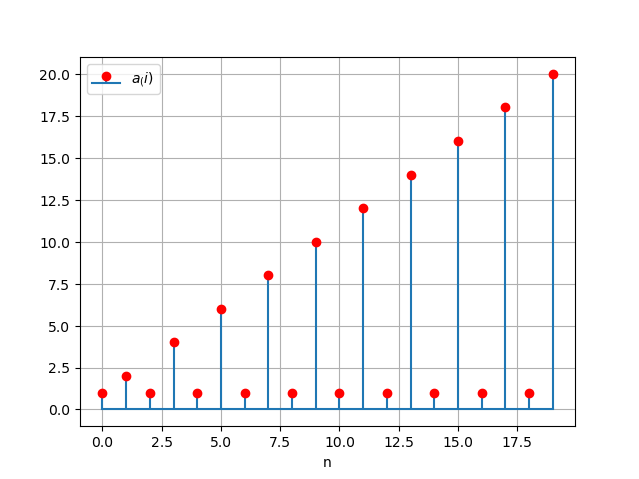
\includegraphics[width = \columnwidth]{figs/Figure_1.png}
    \caption{Terms of the sequence given}
    \centering
    \label{fig: nm_63_fig_2}
\end{figure}
\end{document}

